%
% CS 321: Wed Oct  9 12:07:53 PDT 2013
%
\documentclass[12pt]{article}

\usepackage{amsmath}
\usepackage{amssymb}
\usepackage{amsthm}

\usepackage{geometry}

\usepackage{tikz}
\usetikzlibrary{arrows,automata}

\title{CS321 - Notes}
\author{Trevor Bramwell}
\date{\today}

\begin{document}
\maketitle

\section*{DFAs}

$L = \{ w : w \in \{a, b\}^*,$ each $a$ is preceeded by a $b \}$.

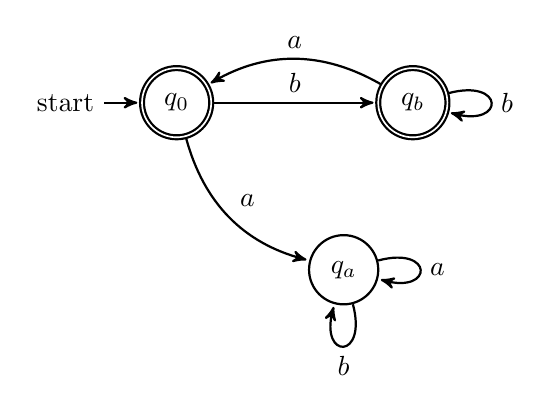
\begin{tikzpicture}[->,>=stealth',shorten >=1pt,auto,node distance=3cm,
                    thick]
  \tikzstyle{every state}=[fill=white]

  \node[state,initial,accepting]   (A)              {$q_0$};
  \node[state,accepting]           (B) [right of=A] {$q_b$};
  \node[state]                     (C) [below right of=A] {$q_a$};

  \path (A) edge              node {$b$} (B)
            edge [bend right] node {$a$} (C)
        (B) edge [loop right] node {$b$} (B)
            edge [bend right] node [above] {$a$} (A)
        (C) edge [loop right] node {$a$} (C)
            edge [loop below] node {$b$} (C);

\end{tikzpicture}

\section*{NFAs (Non-deterministic Finite Acceptors)}

Quantum computers at a first level of approximation, you solve a problem
by trying all possible solutions at the same time. This is sorta what
non-determinism is.

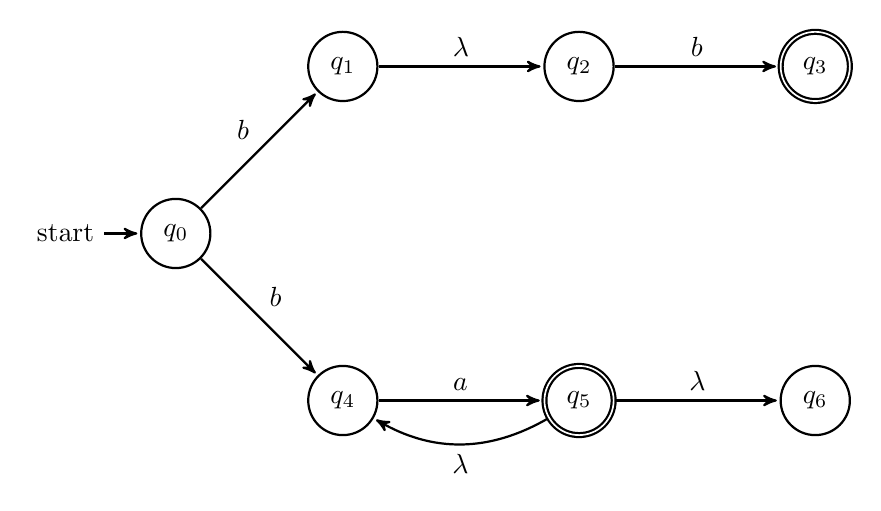
\begin{tikzpicture}[->,>=stealth',shorten >=1pt,auto,node distance=3cm,
                    thick]
  \tikzstyle{every state}=[fill=white]

  \node[state,initial]   (A)              {$q_0$};
  \node[state]           (B) [above right of=A] {$q_1$};
  \node[state]                     (C) [right of=B] {$q_2$};
  \node[state,accepting]                     (D) [right of=C] {$q_3$};
  \node[state]                     (E) [below right of=A] {$q_4$};
  \node[state,accepting]                     (F) [right of=E] {$q_5$};
  \node[state]                     (G) [right of=F] {$q_6$};

  \path (A) edge node {$b$} (B)
            edge node {$b$} (E)
        (B) edge node {$\lambda$} (C)
        (C) edge node {$b$} (D)        
        (E) edge node {$a$} (F)
        (F) edge [bend left] node {$\lambda$} (E)
            edge node {$\lambda$} (G);
\end{tikzpicture}


\subsection*{Acceptance Criterial for Strings}
$L(N)$ what is the language for an NFA $N$?

NFAs accept a string $w$ only if:
\begin{enumerate}
    \item $w$ can be completely read in.
    \item $w$ ends up a in an accept state.
\end{enumerate}
Since we are working with NFAs, $w$ can take all paths at once. 
In order for $w$ to be accepted by the NFA, only one of the paths
has to end in an accept state.

\subsubsection*{Examples}

\begin{itemize}
    \item $w = abb$, reject.
    \item $w = baa$, accept, though the NFA can also reject it.
    \item $w = bbb$, reject, because the NFA will never read in
                     a 3rd b after $q_3$.
\end{itemize}

\subsection*{Powersets}

Let $Q$ be a set.
The power set of $Q$ (written $2^Q$) is a set that contains
all subsets of $Q$.

\subsubsection*{Example}
\begin{align*}
    Q &= \{1, 2, 3\}.\\
  2^Q &= \{ \emptyset, \{1\}, \{2\}, \{3\}, \{1,2\}, \{2,3\}, \ldots \}.
\end{align*}

\subsection*{NFA as a 5-Tuple}
An NFA is a 5-tuple. It can be written as:

\begin{equation*}
    (Q, \Sigma, \delta, q_0, F)
\end{equation*}
where $Q, \Sigma, q_0,$ and $F$ are as for DFA, and 
\begin{equation*}
    \delta : Q \times (\Sigma \cup \{\lambda\}) \to 2^Q.
    % or is it \Sigma^Q?
\end{equation*}

The transition function is: $\delta(q, a) = Q'$. Given the state $q$,
and the string $a$, $Q' \subseteq Q$, where $Q$ is all possible states
- as with DFAs.

\subsection*{Examples}

\begin{align*}
    \delta(q_0, b) &= \{q_1, q_4\} \\
    \delta(q_0, a) &= \emptyset \\
    \delta(q_5, \lambda) &= \{q_4, q_6\}
\end{align*}

$\delta^*(q, w)$ is the set of states that are reachable starting from
$q$ and reading \emph{all} of $w$.

\begin{align*}
    \delta^*(q_0, \lambda) &= \{q_0\}\\
    \delta^*(q_1, \lambda) &= \{q_1, q_2\}\\
    %\delta^*(q_2, \lambda) &= \{q_4, q_3, q_2\}\\
    \delta^*(q_2, \lambda) &= \{q_2\}\\
    \delta^*(q_0, b) &= \{q_1, q_2, q_4\}\\
    \delta^*(q_1, bbb) &= \emptyset
\end{align*}

\end{document}
